Das Generic Attribute Profile (GATT) dient zur Kommunikation zwischen Client und Server. Es basiert auf dem Attribute Protocol (ATT), welches ausgehend vom Server Attribute bereitstellt, die von einem oder mehreren Clients entdeckt werden können. Ein Attribut besteht aus einem Typ, der anhand des Universal Unique Identifier (UUID) identifiziert wird, einem Attribute Handle, um auf das Attribut zuzugreifen, und einem Wert, der von Server und Client ausgelesen bzw. überschrieben werden kann. Zudem ist es möglich für Attribute Berechtigungen festzulegen (bspw. nur Lesen, nicht Schreiben). \cite{BtSpec4.0_1835}
% QUELLE Spec 4.0 S. 1835 3.1 Introduction

Entsprechend der S. \pageref{fig: host controller architektur} Abb. \ref{fig: host controller architektur} ordnet sich ATT über L2CAP in den Protokollstapel ein.

Möchte ein Client einen Attributwert lesen bzw. schreiben, dann sendet er eine Read Request bzw. eine Write Request an den Server. Dieser reagiert, indem er bei einer Read Request das Attribut an den Client sendet oder bei einer Write Request den Attributwert entsprechend ändert und dem Client eine Bestätigung sendet. Im Fall, dass ausgehend vom Server ein Attribut geändert werden soll, sendet dieser eine Notification oder eine Indication an den Client. Im Gegensatz zur Notification wird eine Indication vom Client bestätigt, falls diese empfangen wurde. \cite{BtSpec4.0_1854-1855} \cite{BtSpec4.0_1861-1863}
% QUELLE Spec 4.0 S. 1854 f. 3.4.4.3 Read Request und 3.4.4.4 Read Response
% QUELLE Spec 4.0 S. 1861-1863 3.4.5.1 Write Request und 3.4.5.2 Write Response

Die Daten werden in Form von Attribute Protocol PDUs (siehe Abb. \ref{fig: att pdu}) übertragen.

\begin{figure}[H]
    \centering
    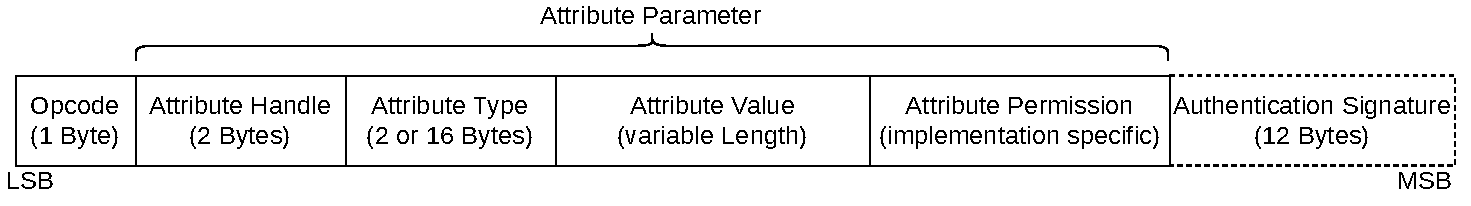
\includegraphics[width=0.9\textwidth]{graphics/att_pdu.pdf}
    \caption[(Generic) Attribute Protocol PDU]{(Generic) Attribute Protocol PDU; in Anlehnung an \cite{BtSpec4.0_fig_1888} und \cite{BtSpec4.0_fig_1889}}
    \label{fig: att pdu}
\end{figure}
% Quelle Spec 4.0 S. 1888 Figure 2.3 und S. 1889 Firgure 2.4

Der ein Byte lange Opcode sagt aus, ob die PDU entweder eine Request, Response, Notification, Indication oder Bestätigung ist, und enthält eine Flag für die Authentifizierung. Die Attributparameter unterteilen sich in zwei Byte für den Attribute Handle, 2 oder 16 Byte für den Attribute Type also die UUID, den Attributwert variabler Länge und die Attributberechtigungen, deren Länge von der Implementierung abhängig ist. Auf die Attributparameter folgt die 12 Byte lange Signatur für die Authentifizierung, falls diese gefordert wird. \cite{BtSpec4.0_1888-1889}
% QUELLE Spec 4.0 S. 1888 f.
\\\\

\begin{figure}{H}
    \centering
    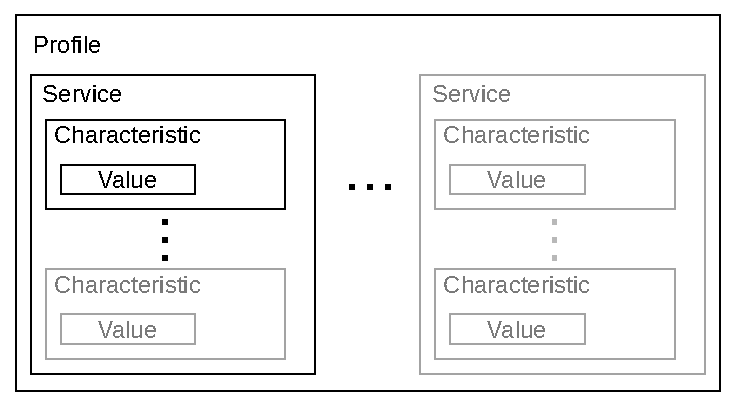
\includegraphics[width=0.9\textwidth]{graphics/gatt_hierarchie.pdf}
    \caption[]{\cite{BtSpec4.0_fig_1892}}
    \label{fig: gatt hierarchie}
\end{figure}
% Quelle Spec 4.0 S. 1892

GATT bildet eine Hierachie (siehe Abb. \ref{fig: gatt hierarchie}) bestehend aus den grundlegenden Elementen Profile, Service und Characteristic, die alle als Attribute definiert werden. An oberster Stelle befindet sich das Profile. Dieses enthält einen oder mehrere Services. Ein Service kann wiederum eine oder mehrere Characteristics enthalten, die sich aus Properties, einem Wert und Descriptors zusammensetzen.